%   ------------------------------------------------------------------------
\FloatBarrier
\subsection{Ferramenta de animação para animação}
\label{s.pixelLab.animacao}

A ferramenta de animation to animation (animação para animação, em inglês) utiliza o sprite de uma pessoa e uma animação qualquer como referências para animar o movimento desse personagem. A funcionalidade pode gerar até 15 frames e também usa uma descrição do personagem a ser animado e da ação a ser feita, com opções de customização do contorno e shading (sombreamento, em inglês) que o resultado final deve ter. A  funcionalidade de limitação de cores considera a paleta do primeiro frame da animação de base, e não do sprite de referência. Existem também duas variáveis que influenciam a geração: AI freedom (liberdade da IA, em inglês), que determina o quanto a IA deve imitar a animação de referência; e guidance weight (peso da orientação, em inglês), que indica o quanto a descrição influencia no resultado.

O objetivo da primeira bateria de testes dessa funcionalidade foi gerar uma animação do personagem Pablo andando, utilizando como base o sprite sheet gerado pela ferramenta God Mode AI (Figura \ref{fig:pixelLabSpriteSheetGodModeAI}). Antes de ser usada como referência, a imagem gerada pela ferramenta Gemini Pro (detalhada na Seção \ref{s.ferramentaB}) do personagem Pablo em side view (Figura \ref{fig:pixelLabPabloGeminiProSide}) passou por ajustes finos, como pode ser visto na Figura \ref{fig:pixelLabAniSideViewSprite1}. É importante notar que este sprite representa uma versão intermediária do resultado final da edição. Análises posteriores levaram a um refinamento adicional, cujo processo é detalhado na Seção \ref{s.pixelLab.edicao}, resultando na versão final utilizada no jogo.

\begin{figure}[htbp]
    \centering
    \caption{\small Sprite do personagem em side view após ajuste fino}
    \label{fig:pixelLabAniSideViewSprite1}
    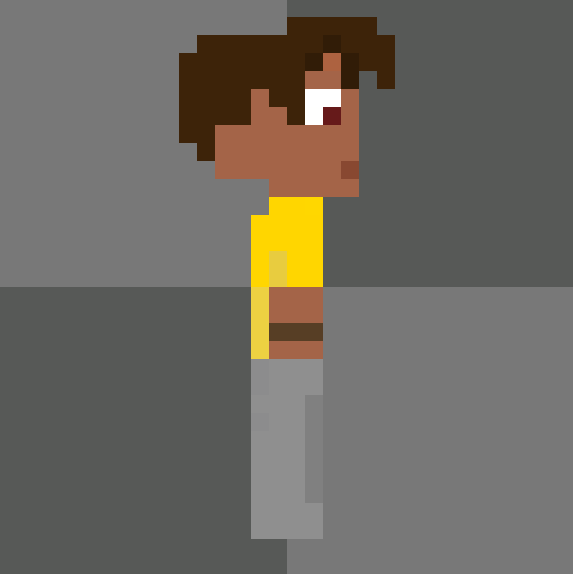
\includegraphics[width=0.4\linewidth]{figs/pixelLab/dia3/fixGrande.PNG}
    \legend{\small Fonte: Elaborada pela autora.}
\end{figure}

Durante o teste inicial, a imagem corrigida e a animação citada anteriormente são colocadas como referência, enquanto é utilizado um prompt simples que descreve as roupas usadas pelo personagem, como pode ser verificado na Figura \ref{fig:pixelLabAniTela}.


\begin{figure}[htbp]
    \centering
    \caption{\small Tela da geração de animação no Pixel Lab}
    \label{fig:pixelLabAniTela}
    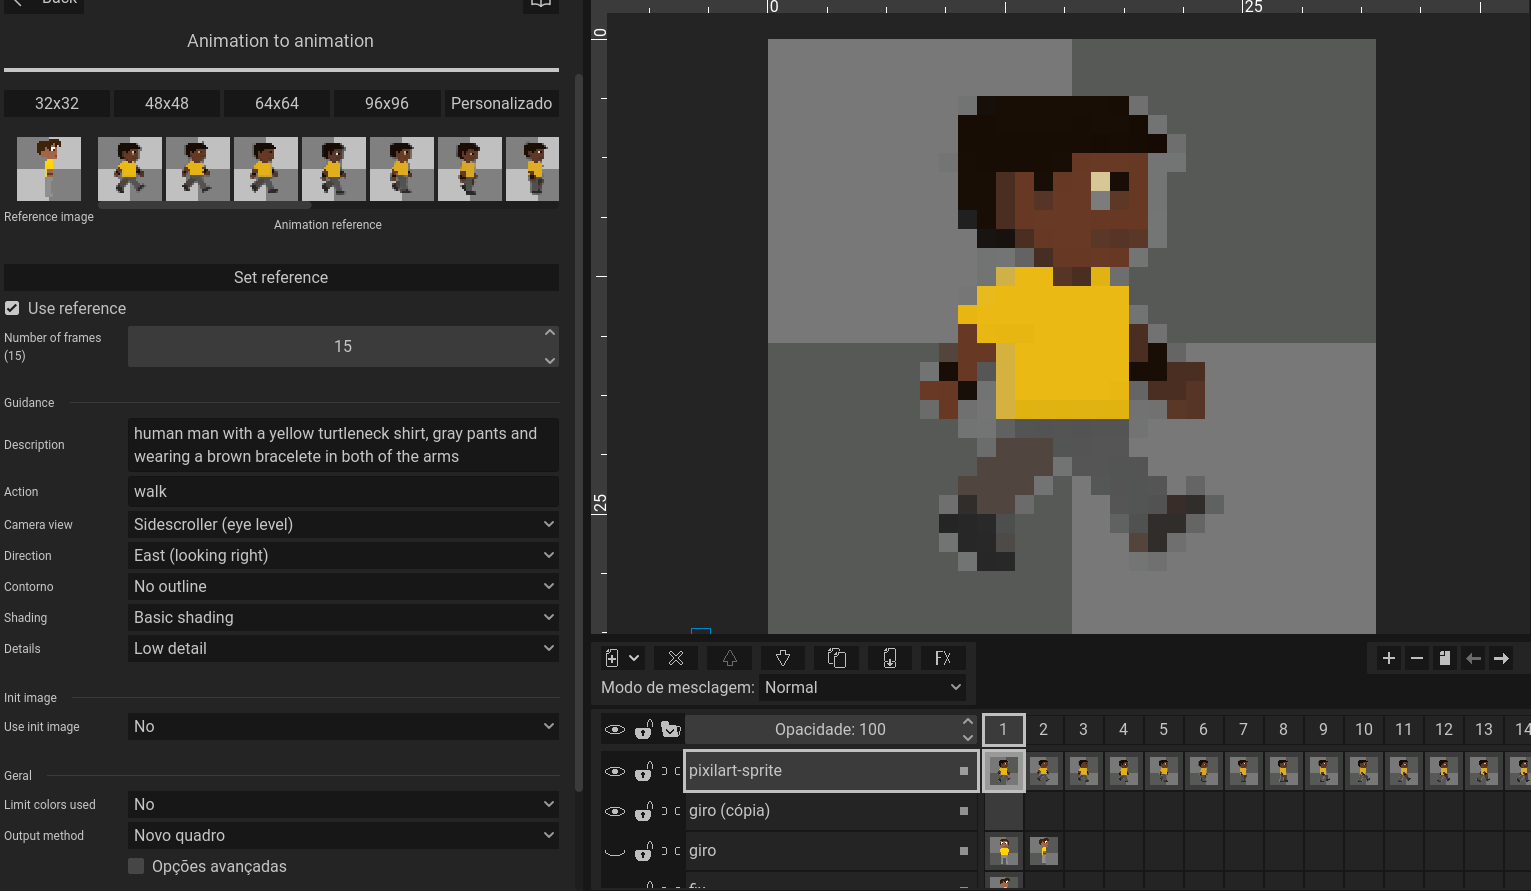
\includegraphics[width=1\linewidth]{figs/pixelLab/dia3/tela_animacao.PNG}
    \legend{\small Fonte: Elaborada pela autora.}
\end{figure}

O resultado gerado\footnote{\url{https://drive.google.com/file/d/1TYecwF1D5EqbKaJIOJle_iZbkVOuWsux/view?usp=sharing}} foi insatisfatório, apresentando uma aparência diferente do personagem de referência, além de não possuir o mesmo estilo de pixel art, como pode ser visto na Figura \ref{fig:pixelLabAniResRuim}.

\begin{figure}[htbp]
    \centering
    \caption{\small Quadro da animação gerada no Pixel Lab}
    \label{fig:pixelLabAniResRuim}
    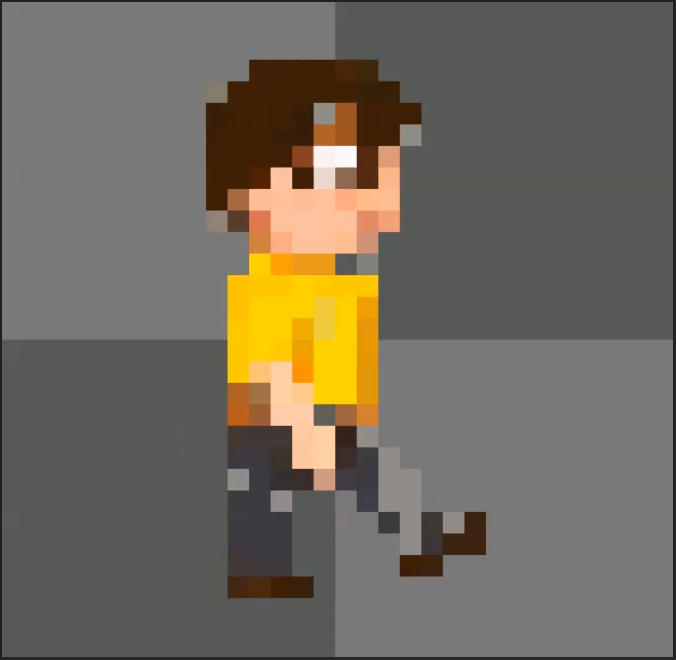
\includegraphics[width=0.4\linewidth]{figs/pixelLab/dia3/print1.PNG}
    \legend{\small Fonte: Elaborada pela autora.}
\end{figure}

Levando em conta esse erro, em testes posteriores foi adicionada a descrição da aparência do personagem no prompt como pode ser verificado na Figura \ref{fig:pixelLabAniPrompt}. Durante cada uma das interações, algumas palavras do prompt e as configurações de sombreamento são mudadas, visando obter um resultado mais consistente com o sprite de referência. As tentativas completas podem ser consultadas nas Figuras \ref{fig:pixelLabAnimacao1} a \ref{fig:pixelLabAnimacao6} do Apêndice \ref{ap.telasIA}. 

\begin{figure}[htbp]
    \centering
    \caption{\small Prompt com a descrição da aparência}
    \label{fig:pixelLabAniPrompt}
    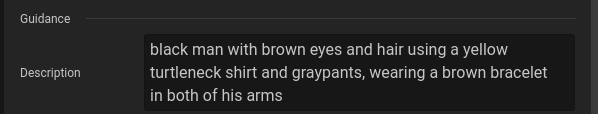
\includegraphics[width=0.7\linewidth]{figs/pixelLab/dia3/prompt.PNG}
    \legend{\small Fonte: Elaborada pela autora.}
\end{figure}

A geração de uma animação possui o mesmo processo da geração de imagem, o que faz sentido considerando que um vídeo é formado por várias figuras (quadros). 

Durante um dos testes, ocorreu algo inesperado: nenhuma animação foi gerada. Investigando mais a fundo, foi descoberto que, na última etapa do processamento, onde o fundo deveria ser removido, o sprite inteiro foi deletado. Esse erro não se repetiu em mais nenhum outro teste. Abaixo se encontram as Figuras \ref{fig:pixelLabAniPromptFalha} e \ref{fig:pixelLabAniTelaFalha} mostrando o prompt usado e o resultado gerado na interação falha.


\begin{figure}[htbp]
    \centering
    \caption{\small Prompt que gerou a falha no Pixel Lab}
    \label{fig:pixelLabAniPromptFalha}
    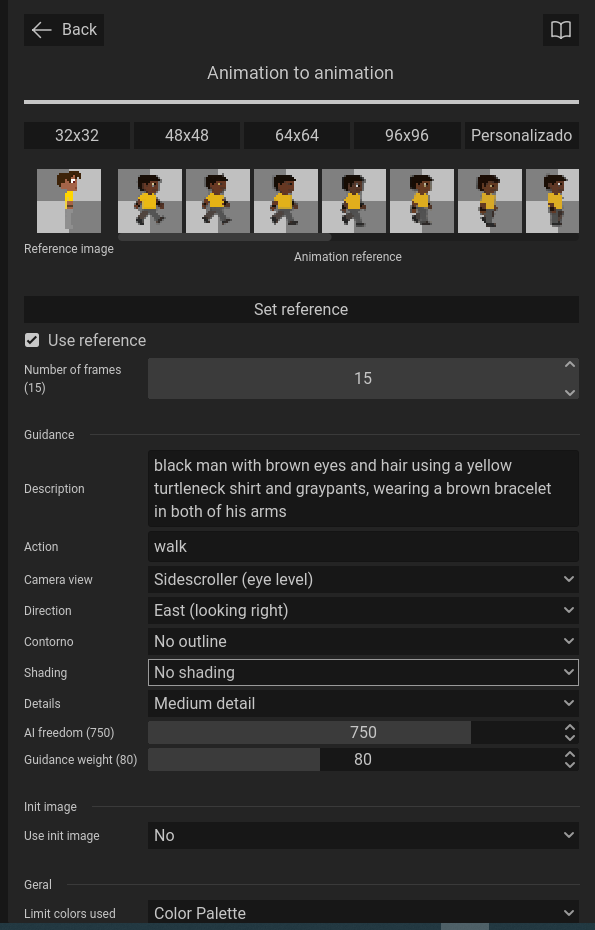
\includegraphics[width=0.53\linewidth]{figs/pixelLab/dia3/tela_3.PNG}
    \legend{\small Fonte: Elaborada pela autora.}
\end{figure}

\begin{figure}[htbp]
    \centering
    \caption{\small Quadros vazios após a geração no Pixel Lab}
    \label{fig:pixelLabAniTelaFalha}
    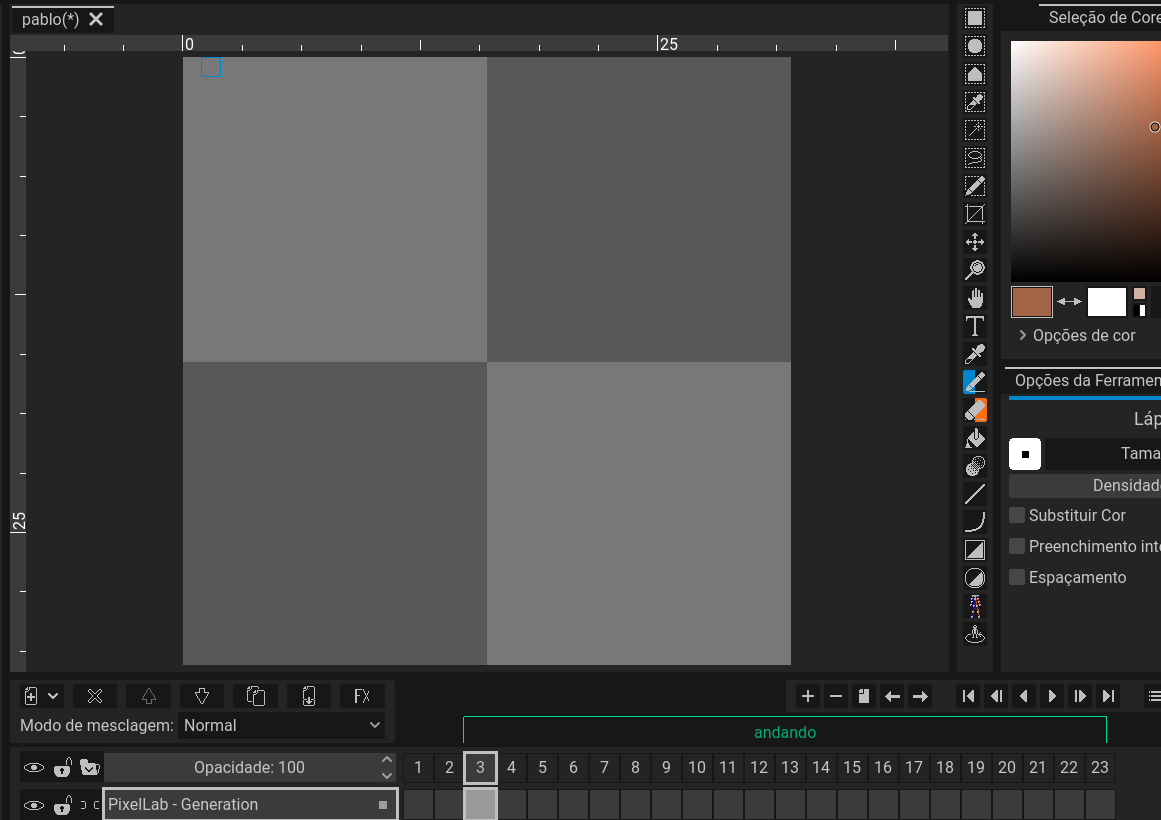
\includegraphics[width=0.7\linewidth]{figs/pixelLab/dia3/falha3.PNG}
    \legend{\small Fonte: Elaborada pela autora.}
\end{figure}

Analisando os resultados, nenhum deles manteve o formato da silhueta original, os tons de cores ficaram levemente distintos do personagem a ser animado e possuíam falhas de pixels que tornavam as características do rosto menos reconhecíveis. Foi possível notar que o tamanho e a forma do sprite da animação de referência influenciaram as imagens geradas, o que pode ser observado mais atentamente na Figura \ref{fig:pixelLabAnimaCompara}. Investigando mais a fundo, isso acontece por causa do funcionamento da funcionalidade animação para animação, que cria o esqueleto da animação de referência, e usa a movimentação que o esqueleto apresentou para criar uma nova animação. O esqueleto da animação de base mantém o formato e o tamanho da mesma, e o resultado final é gerado por cima desse esqueleto, utilizando as características deste.

\begin{figure}[htbp]
    \centering
    \caption{\small Comparação do sprite original com os frames da animação de base e da gerada no Pixel Lab}
    \label{fig:pixelLabAnimaCompara}

    \begin{subfigure}{0.32\linewidth}
        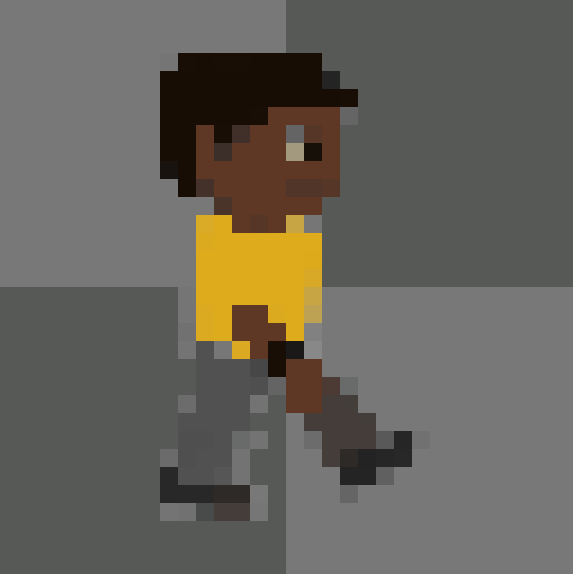
\includegraphics[width=0.9\linewidth]{figs/pixelLab/dia3/print0.PNG}
        \caption{\small Frames da animação de referência}
        \label{fig:pixelLabAnimaComparaAni}
    \end{subfigure}
    \begin{subfigure}{0.32\linewidth}
        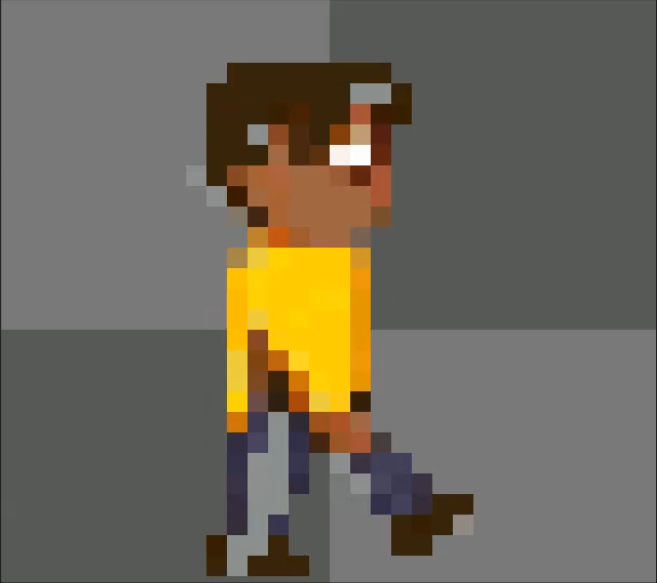
\includegraphics[width=1\linewidth]{figs/pixelLab/dia3/print4.PNG}
        \caption{\small Frame da animação gerada }
        \label{fig:pixelLabAnimaComparaGera}
    \end{subfigure}
    \begin{subfigure}{0.32\linewidth}
        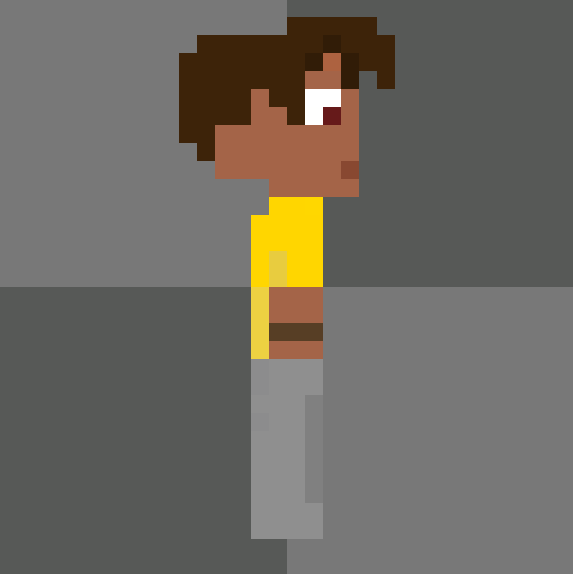
\includegraphics[width=0.9\linewidth]{figs/pixelLab/dia3/fixGrande.PNG}
        \caption{\small Sprite original em side view }
        \label{fig:pixelLabAnimaComparaSprite}
    \end{subfigure}
    \legend{\small Fonte: Elaborada pela autora, utilizando a ferramenta Pixel Lab.}
\end{figure}


A análise mostra que usar a ferramenta com uma animação que não é consistente com o sprite em tamanho e formato não gera resultados satisfatórios que possam ser aplicados em um jogo. Considerando esse fator, posteriormente foi realizada uma segunda bateria de testes, utilizando para a geração da nova animação o sprite sheet do vídeo do personagem Pablo andando gerado pela ferramenta Gemini Pro (Figura \ref{fig:pixelLabSpriteSheetGeminiPro}), que possui características extremamente próximas ao sprite original, porém apresenta pequenos erros. Além disso, como imagem de referência será usada a versão final do ajuste fino do sprite do personagem Pablo em side view gerado pelo Gemini Pro (Figura \ref{fig:pixelLabAniSideViewSprite2}).

\begin{figure}[htbp]
    \centering
    \caption{\small Quadro da animação gerada no Pixel Lab}
    \label{fig:pixelLabAniSideViewSprite2}
    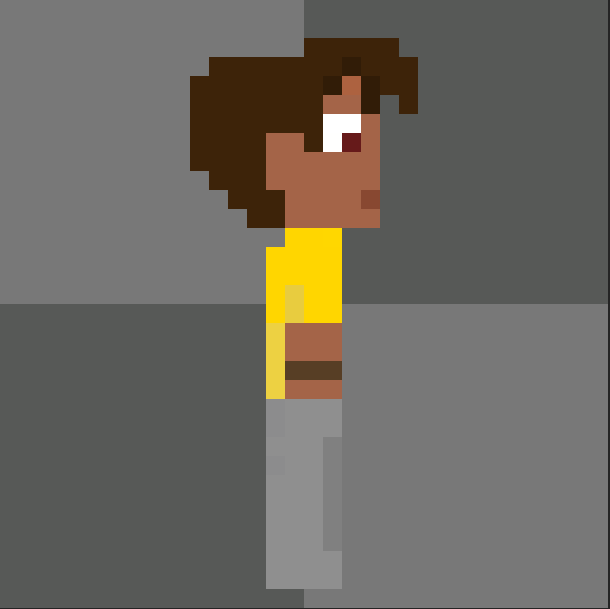
\includegraphics[width=0.4\linewidth]{figs/pixelLab/dia3/fix_oficial_fundo_igual.PNG}
    \legend{\small Fonte: Elaborada pela autora.}
\end{figure}

Os resultados\footnote{\url{https://drive.google.com/drive/folders/1xmE-wpvT9xLguyX2izbWv2Xn0glh84IZ?usp=sharing}} gerados obtiveram uma alta consistência, porém a qualidade deles foi menor do que a da animação de referência, com tons de cores diferentes do sprite original e erros nos pixels, porém possuindo o formato mais preciso da mão, como pode ser visto na Figura \ref{fig:pixelLabAnimaComparaGemini}. A interação completa pode ser consultada nas Figuras \ref{fig:pixelLabAnimacao7} e \ref{fig:pixelLabAnimacao8} do Apêndice \ref{ap.telasIA}. 

\begin{figure}[htbp]
    \centering
    \caption{\small Comparação do sprite de referência com os frames da animação de base e da gerada no Pixel Lab}
    \label{fig:pixelLabAnimaComparaGemini}

    \begin{subfigure}{0.32\linewidth}
        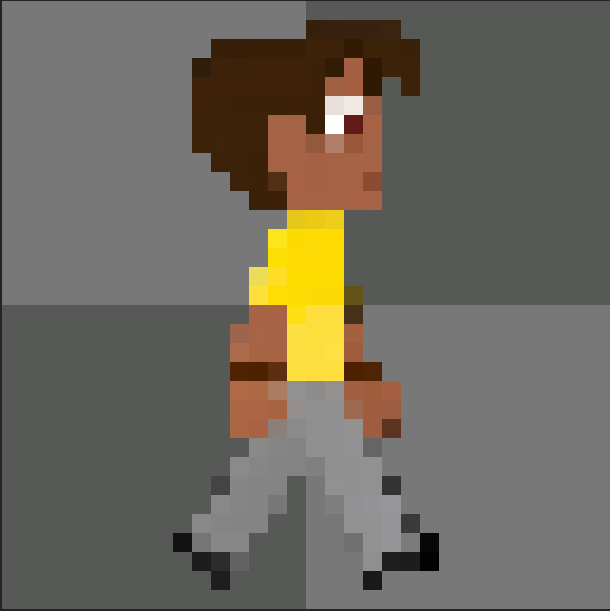
\includegraphics[width=1\linewidth]{figs/pixelLab/dia4/print0.PNG}
        \caption{\small Frame da animação de referência, com cores mais precisas e dedão na mão visível}
        \label{fig:pixelLabAnimaComparaGeminiAni}
    \end{subfigure}
    \begin{subfigure}{0.32\linewidth}
        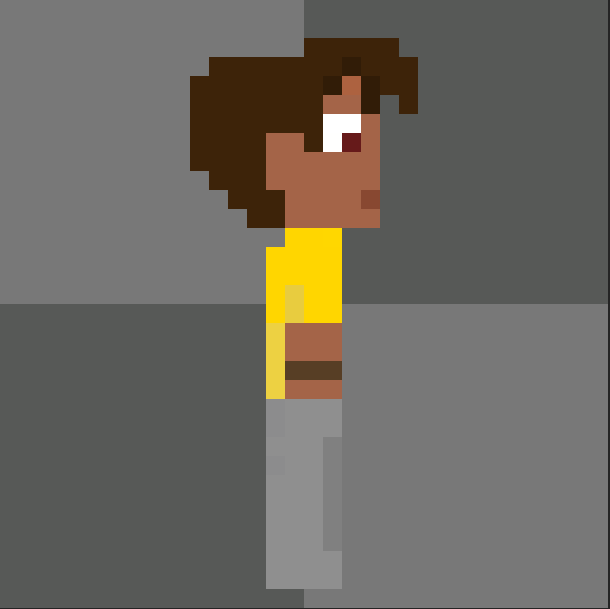
\includegraphics[width=1\linewidth]{figs/pixelLab/dia3/fix_oficial_fundo_igual.PNG}
        \caption{\small Sprite de referência em side view, sem dedão visível na mão}
        \label{fig:pixelLabAnimaComparaGeminiSprite}
    \end{subfigure}
    \begin{subfigure}{0.32\linewidth}
        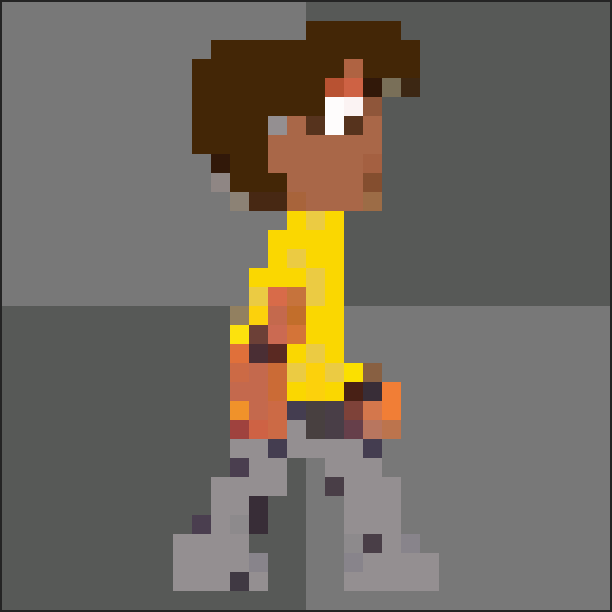
\includegraphics[width=1\linewidth]{figs/pixelLab/dia4/print1.PNG}
        \caption{\small Frame da animação gerada, com cores menos precisas e sem dedão na mão}
        \label{fig:pixelLabAnimaComparaGeminiGera}
    \end{subfigure}
    \legend{\small Fonte: Elaborada pela autora, utilizando a ferramenta Pixel Lab.}
\end{figure}

Nos testes posteriores, além de se utilizar a opção de limitar as cores da animação gerada de acordo com a paleta do primeiro frame, o mesmo foi editado para ter as cores exatas do sprite original. O objetivo era testar a capacidade da ferramenta na geração da animação, sem buscar apenas produzir uma animação melhor pela edição manual. Como a animação mostrada parcialmente na Figura \ref{fig:pixelLabAnimaComparaGeminiGera}, apesar de ter tons de cores diferentes, possui um formato mais preciso, ela também foi utilizada como referência após a do sprite original como primeiro quadro. 

Os resultados\footnote{\url{https://drive.google.com/drive/folders/1YHiklOXkW1FhYC_fBS00c21wt8fMNiIq?usp=drive_link}} obtiveram uma queda na qualidade, com as cores sendo utilizadas de maneira imprecisa e possuindo ainda mais erros nos pixels, como pode ser visto na Figura \ref{fig:pixelLabAnimaComparaGemini2}. Interações completas podem ser consultadas nas Figuras \ref{fig:pixelLabAnimacao9} a \ref{fig:pixelLabAnimacao11} no Apêndice \ref{ap.telasIA}. Investigando mais a fundo, é descoberto que esse declínio provavelmente foi causado pelo fato de que o sprite original não possui tons suficientes para trazer um efeito de profundidade na região das pernas e dos braços, fazendo a IA aplicar cores totalmente diferentes em regiões que precisam ter essa diferença.

\begin{figure}[htbp]
    \centering
    \caption{\small Comparação do sprite de referência com os frames das animações geradas no Pixel Lab}
    \label{fig:pixelLabAnimaComparaGemini2}

    \begin{subfigure}{0.32\linewidth}
        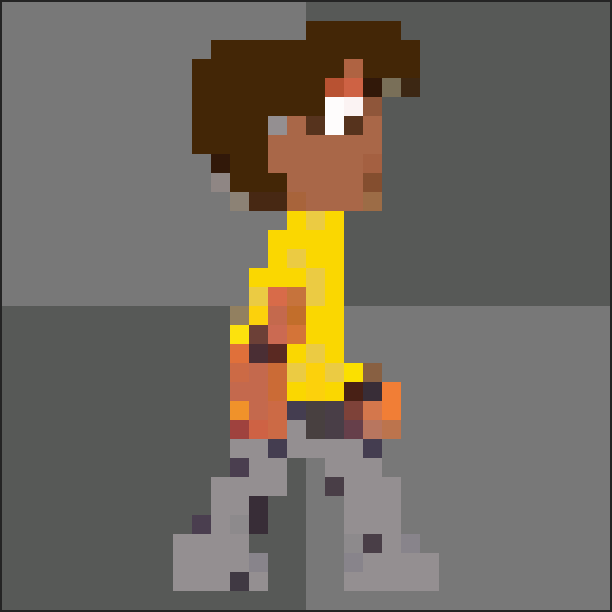
\includegraphics[width=1\linewidth]{figs/pixelLab/dia4/print1.PNG}
        \caption{\small Frame da animação gerada sem limitar as cores para apenas as mesmas do sprite de referência}
        \label{fig:pixelLabAnimaComparaGeminiAni2}
    \end{subfigure}
    \begin{subfigure}{0.32\linewidth}
        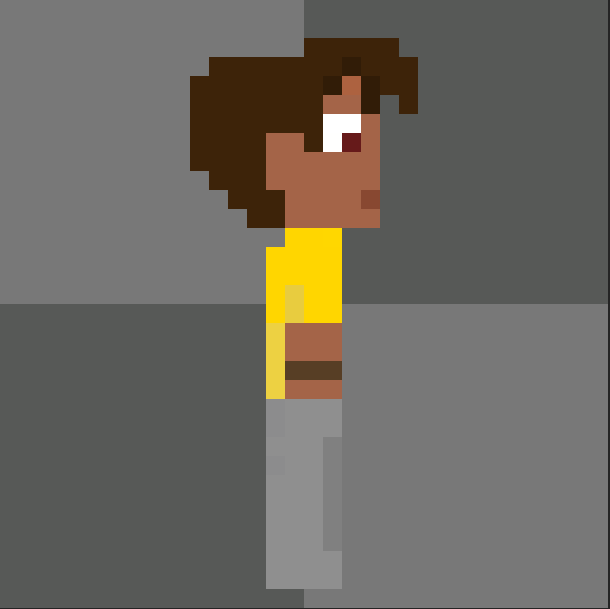
\includegraphics[width=1\linewidth]{figs/pixelLab/dia3/fix_oficial_fundo_igual.PNG}
        \caption{\small Sprite de referência em side view}
        \label{fig:pixelLabAnimaComparaGeminiSprite2}
    \end{subfigure}
    \begin{subfigure}{0.32\linewidth}
        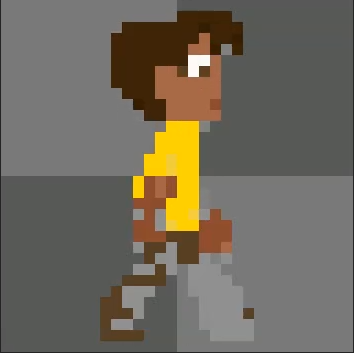
\includegraphics[width=1\linewidth]{figs/pixelLab/dia4/print6.PNG}
        \caption{\small Frame da animação gerada limitando as cores para apenas as mesmas do sprite de referência}
        \label{fig:pixelLabAnimaComparaGeminiGera2}
    \end{subfigure}
    \legend{\small Fonte: Elaborada pela autora, utilizando a ferramenta Pixel Lab.}
\end{figure}

Para explorar os limites da ferramenta, foi conduzido um último teste. O objetivo era verificar se essa funcionalidade também poderia ser utilizada para gerar uma animação de rotação completa, uma tarefa normalmente designada à ferramenta de rotação. 

Para isso, foi criada manualmente uma animação de pseudo-rotação utilizando os sprites já existentes do personagem Pablo (visão frontal, lateral, de costas e lateral espelhada), cada um ocupando um quadro para simular um giro de 360 graus. Esta animação serviu como referência de movimento. Como sprite de referência, foi utilizada a personagem Luz, que possui um corpo com proporções e tamanho significativamente diferentes. Naquele momento, ainda não havia sido compreendido totalmente que a animação gerada seguia o formato da animação de referência e não do sprite.

O resultado\footnote{\url{https://drive.google.com/file/d/1NEfmTRU46067ueFgWvvhpd1MQBiyhP1H/view?usp=sharing}} gerado foi completamente insatisfatório, produzindo uma animação completamente deformada que tentava aplicar as proporções maiores do personagem Pablo ao corpo menor da personagem Luz. Este experimento serviu como confirmação definitiva da teoria levantada nos testes anteriores: a ferramenta prioriza a estrutura geométrica e as proporções do esqueleto da animação de referência, em vez de seguir o formato do sprite de referência. A inconsistência dimensional entre os dois inputs leva inevitavelmente a um resultado de baixa precisão, como pode ser visto na Figura \ref{fig:pixelLabAnimaComparaRodarSprite}.

\begin{figure}[htbp]
    \centering
    \caption{\small Comparação do sprite original com os frames da animação gerada no Pixel Lab}
    \label{fig:pixelLabAnimaComparaRodar}

    \begin{subfigure}{0.32\linewidth}
        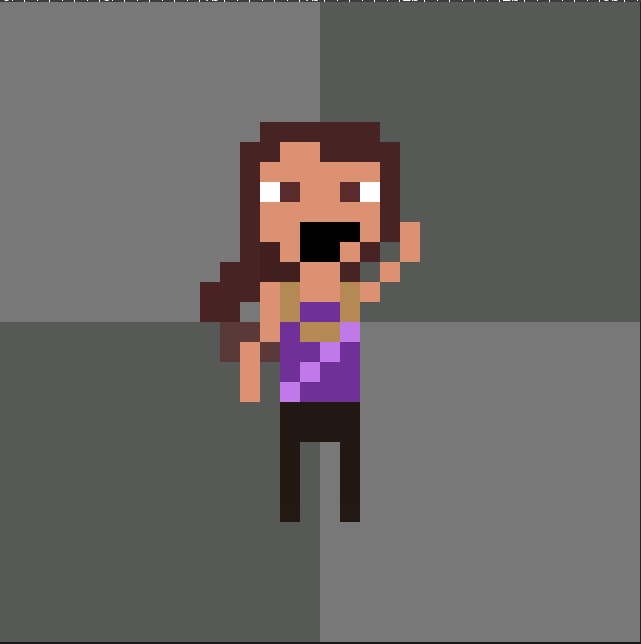
\includegraphics[width=1\linewidth]{figs/pixelLab/dia4/irma.PNG}
        \caption{\small Sprite original}
        \label{fig:pixelLabAnimaComparaRodarSprite}
    \end{subfigure}
    \begin{subfigure}{0.32\linewidth}
        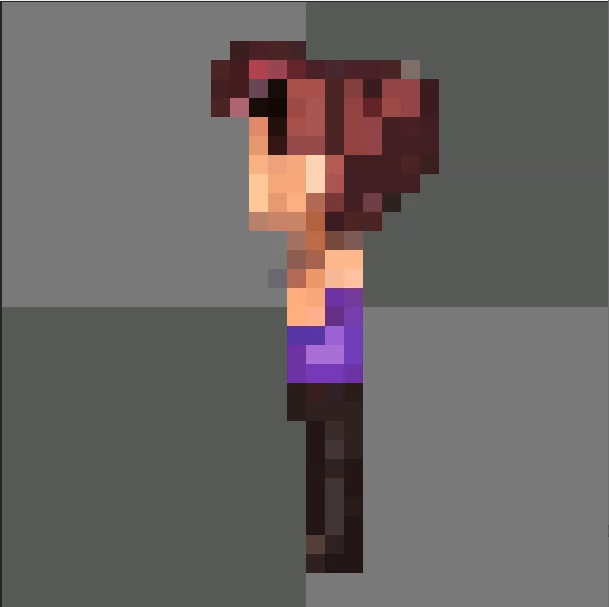
\includegraphics[width=1\linewidth]{figs/pixelLab/dia4/printA.PNG}
        \caption{\small Frame 1 da animação gerada }
        \label{fig:pixelLabAnimaComparaRodarFrame1}
    \end{subfigure}
    \begin{subfigure}{0.32\linewidth}
        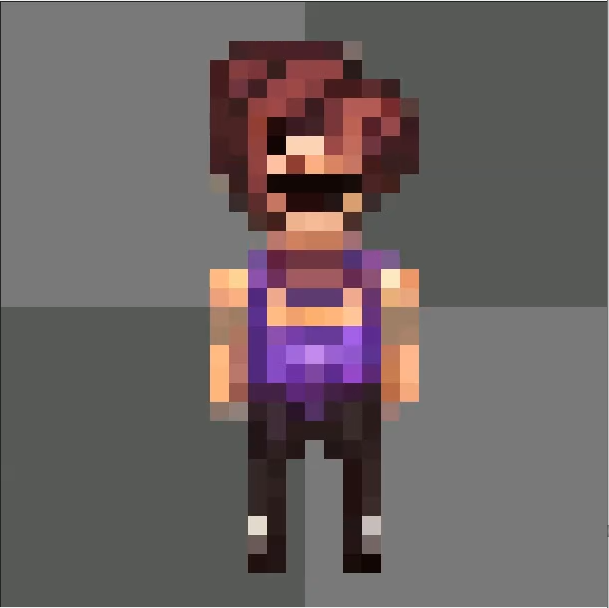
\includegraphics[width=1\linewidth]{figs/pixelLab/dia4/printB.PNG}
        \caption{\small Frame 2 da animação gerada  }
        \label{fig:pixelLabAnimaComparaRodarFrame2}
    \end{subfigure}
    \legend{\small Fonte: Elaborada pela autora, utilizando a ferramenta Pixel Lab.}
\end{figure}

A análise revela que a ferramenta é capaz de gerar animações consistentes se a animação de referência é parecida com o sprite, porém o resultado formado ainda exige ajustes finos, possuindo falhas de pixels e tons de cores não idênticos aos desejados, o que faz com que sua performance na geração não alcance a mesma qualidade comparada às ferramentas descritas nas próximas seções. Apesar disso, assim como a funcionalidade de rotação, a criação de animação baseada em outra animação apresenta grande potencial de otimização do processo em cenário com uma animação base de alta qualidade ou com diversos personagens de tamanho e forma parecidos.

